\chapter{Vehicle architecture}
\qquad \underline{By} : Lukas\\

This chapter aims to describe the vehicle system architecture. As the space craft needs to be able to perform an aerobreak within earth’s atmosphere, the design is relatively constrained towards a space shuttle-related architecture, with a heat shield in the front, some form of lifting devices and a length to diameter ratio greater than 1. As the satellite capturing system GREDER uses needs to be situated in the front of the vehicle and the propellant choices dictated the performance, the tank volumes were defined by mission requirements and the mass budget. After defining the system diameter to be $2.5$ m, the complete system design was basically finalized. The complete 3D-render can be seen in \autoref{3drender}.

\begin{figure}[H]
	\centering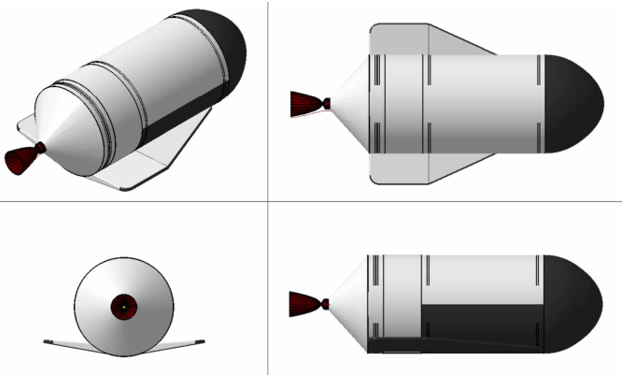
\includegraphics[width=\linewidth]{3drender}
	\caption{Vehicle design 3D-Render}\label{3drender}
\end{figure}

The vehicle consists of 3 zones, which are highlighted in the 3D view as the frontal black zone, the middle white zone and the engine, which is colored in black. The frontal zone houses the battery, fuel cell and capturing equipment as well as the heat shield. A detailed CAD of this area has not been created, as all the equipment was only calculated based on its function and performance. The engine zone, which is the main component of this assignment, will be described in detail, including CAD, calculations and simulations, in \autoref{chap:10} and \autoref{chap:11}. \\

The tank zone, which consists of the oxidizer tank in the upper part of the cylindric vehicle section and the fuel tank in the lower end, is shown in \autoref{vehtank}.

\begin{figure}[H]
	\centering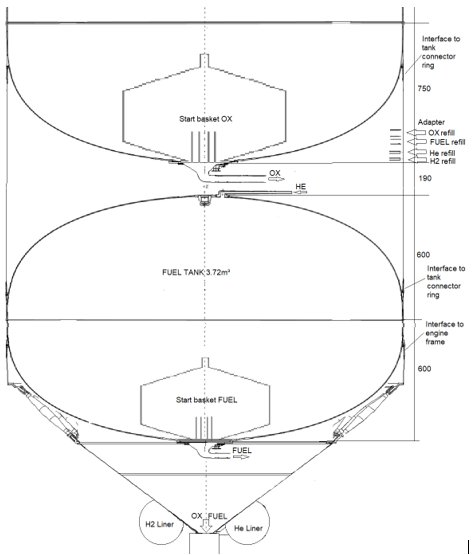
\includegraphics[width=0.8\linewidth]{vehtank}
	\caption{Vehicle architecture - Tank section}\label{vehtank}
\end{figure}

As \autoref{vehtank} shows, the tanks and the outer wall are the same structure throughout the cylindrical sections of the propellant tanks. Both tanks are shapes as cylinders will elliptical bulkheads, between which the oxidizer tank outlet is situated. The refueling ports are located between the tanks as well. The oxidizer as well as liner tank lines are funneled through the wing, which extends down until the engine section, where the engine is structurally supported by a conically shaped engine frame, which is connected to the cylindrical structure by axial dampers.